% Section content template for individual Educative lessons
% This file contains the actual content for a specific section
% Generated from Educative API section content

% Section: AWS Wide Spread Outage
% Section ID: 6672582694141952
% Section Slug: aws-wide-spread-outage
% Generated: 2025-12-08T15:38:10.884068

\subsection{Introduction}\label{FVqL_6vSo2Q8ZMnPSuWGe}
\\
Several Amazon services and other services that depend on AWS were disrupted by an outage incident that spanned more than eight hours on Tuesday, December 7, 2021, at approximately 7:35 a.m. PST. The incident impacted everything from home consumer products to numerous commercial services.
\\
This hours-long outage made headlines in the popular media, such as this one from the \emph{Financial Times}: ``From angry Adele fans to broken robot vacuums: AWS outage ripples through the US.'' The outage affected millions of users worldwide, including individuals who were using the AWS online stores and other businesses that relied heavily on AWS for providing their services.
\\
The disruption caused by AWS emphasized the need for a decentralized Internet where services don't rely on a small number of giant companies. According to Gartner, 80\% of the cloud market is handled by just five companies. Amazon , with a 41\% share of the cloud computing market, is the largest.
\\
Outages like the one above remind us of Lamport's famous quip: ``A distributed system is one in which the failure of a computer you didn't even know existed can render your own computer unusable.''

\subsection{Sequence of events}\label{QeEP2UgNlr9Fo757JyPsc}

\begin{itemize}
\item
\protect\phantomsection\label{YlraTFKzwccMfgpaVgj6m}
An automated action to expand the capacity of one of the AWS services near the main AWS network elicited unusual behavior from a significant number of customers within the internal network.
\item
\protect\phantomsection\label{NYPEQBFI75NjrgNgK9VNR}
As a result, there was a significant increase in connection activity, which swamped the networking equipment that connected the internal network to the main AWS network.
\item
\protect\phantomsection\label{0m9oBJTPmUmNC57afT6Gv}
Communication between these networks got delayed. These delays enhanced latency and failures for services interacting between these networks, leading to a rise in retries and ping requests.
\item
\protect\phantomsection\label{tIW5UtFbWuiFyxW_Yk59h}
As a result, the devices connecting the two networks experienced constant overload and performance difficulties.
\item
\protect\phantomsection\label{60kf0CX74xGmz8pGosGSK}
This overload instantly affected the availability of real-time monitoring data for AWS internal operations teams, hampering their ability to identify and remedy the cause of the congestion.
\item
\protect\phantomsection\label{9HdLzSHGldIMrUBGDxVHR}
Operators relied on logs to figure out what was going on and initially observed heightened internal DNS failures.
\end{itemize}
\\
The following slides show the series of events that led to the outage.

\begin{figure}[htbp]
 \centering
 \begin{subfigure}[b]{0.48\textwidth}
 \centering
 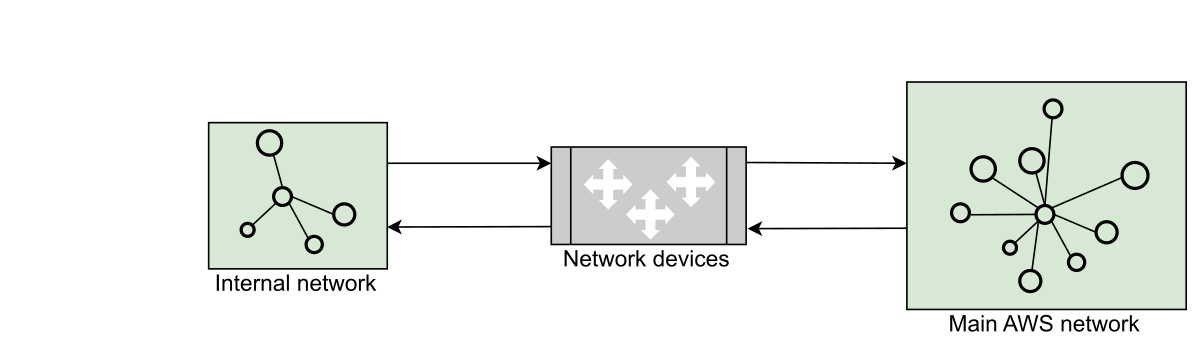
\includegraphics[width=\textwidth]{Images/chapter_42/section_6672582694141952/6567477022818304.png}
 \caption{The high-level infrastructure of Amazon. The main AWS network connects the internal network using networking device}
 \end{subfigure}
 \hfill
 \begin{subfigure}[b]{0.48\textwidth}
 \centering
 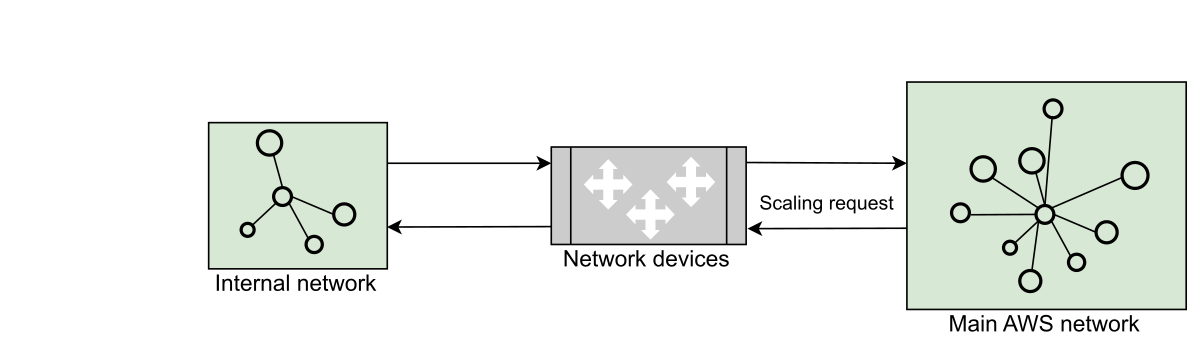
\includegraphics[width=\textwidth]{Images/chapter_42/section_6672582694141952/6150092931465216.png}
 \caption{The main AWS network makes a scaling request to the internal network}
 \end{subfigure}
\end{figure}

\begin{figure}[htbp]
 \centering
 \begin{subfigure}[b]{0.48\textwidth}
 \centering
 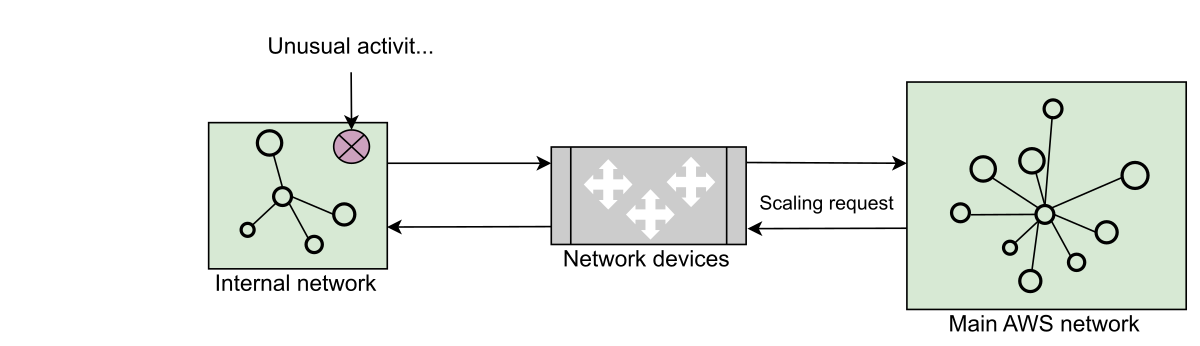
\includegraphics[width=\textwidth]{Images/chapter_42/section_6672582694141952/6462259408928768.png}
 \caption{The scaling request resulted in unusual behavior in the internal network}
 \end{subfigure}
 \hfill
 \begin{subfigure}[b]{0.48\textwidth}
 \centering
 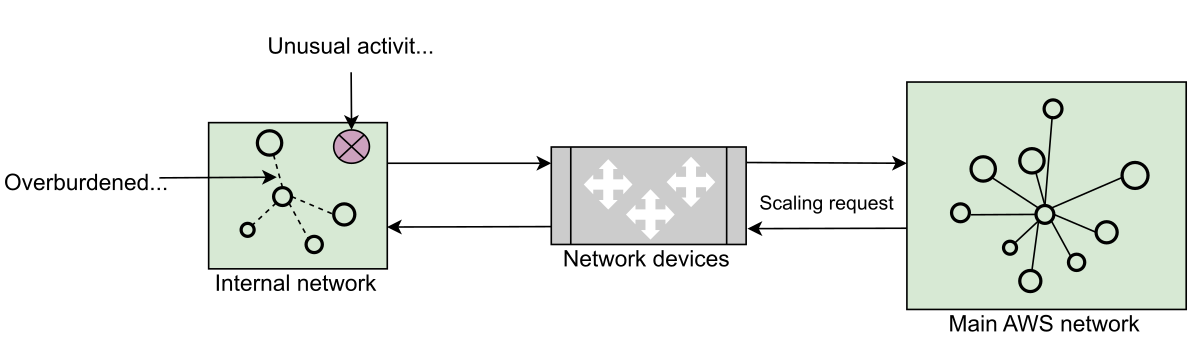
\includegraphics[width=\textwidth]{Images/chapter_42/section_6672582694141952/4632632331862016.png}
 \caption{The internal network received a large number of client requests, which overburdened the network}
 \end{subfigure}
\end{figure}

\begin{figure}[htbp]
 \centering
 \begin{subfigure}[b]{0.48\textwidth}
 \centering
 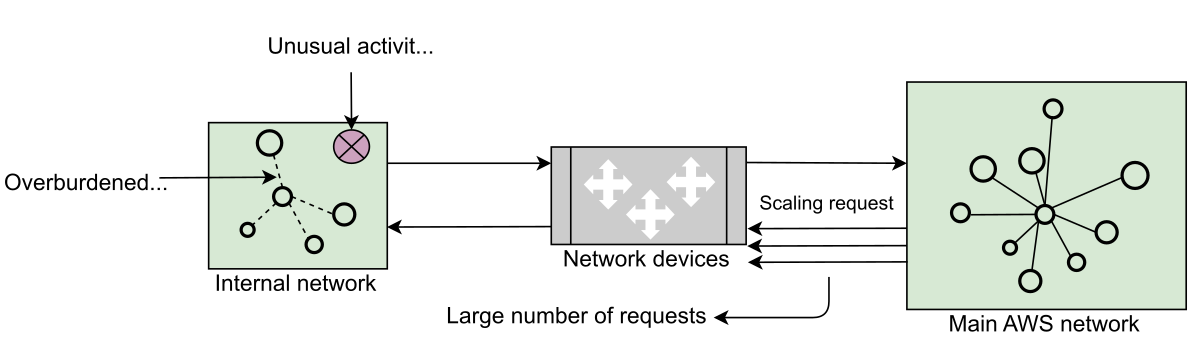
\includegraphics[width=\textwidth]{Images/chapter_42/section_6672582694141952/4612248752619520.png}
 \caption{Additional requests from the main AWS network are received}
 \end{subfigure}
 \hfill
 \begin{subfigure}[b]{0.48\textwidth}
 \centering
 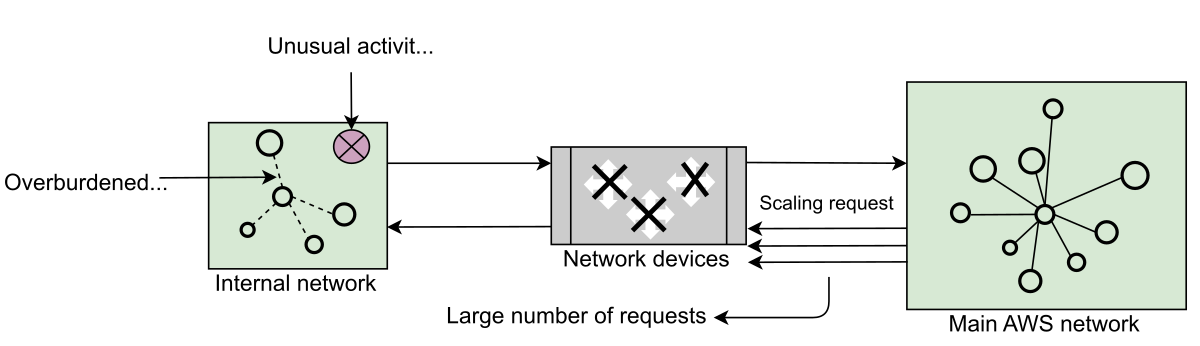
\includegraphics[width=\textwidth]{Images/chapter_42/section_6672582694141952/5905061557567488.png}
 \caption{The network devices become clogged because of a large number of connection requests from main AWS network}
 \end{subfigure}
\end{figure}

\begin{figure}[htbp]
 \centering
 \begin{subfigure}[b]{0.48\textwidth}
 \centering
 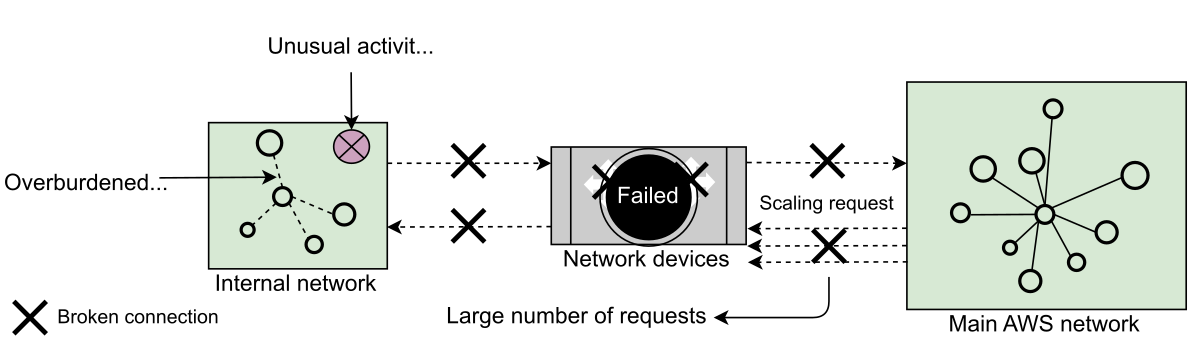
\includegraphics[width=\textwidth]{Images/chapter_42/section_6672582694141952/6647826423742464.png}
 \caption{The network devices fail, which leads to disabled communication between the internal and main AWS networks}
 \end{subfigure}
\end{figure}

\subsection{Analysis}\label{PjXVGxwDQKYmp8RwjZgrb}

\begin{itemize}
\item
\protect\phantomsection\label{D5hQ16r9z_q1dfFl77X20}
\textbf{Hampered AWS services}: The networking difficulties affected a variety of AWS services, impacting customers who utilized these service capabilities. Since the primary AWS network remained unaffected, certain client applications that don't depend on these capabilities suffered relatively minor consequences as a result of this occurrence. AWS users, such as Amazon RDS, EMR, and Workspaces, were unable to generate new resources due to the inability of the system to launch new EC2 instances.
\item
\protect\phantomsection\label{p4WVk6rtxQ3b7otUZ1EpC}
\textbf{Impaired control plane}: Apart from the AWS services, the AWS control planes that are used for establishing and managing AWS resources were also impacted. These control planes take advantage of internal network-hosted services. For example, EC2 instances weren't affected by this event, but EC2 APIs suffered from increased latency and error rates.
\item
\protect\phantomsection\label{rkj_HSUVvqjeKr1fYyXu3}
\textbf{Slow restoration}: Since DNS is the basis for all communication across the web, operators focused on moving the internal DNS traffic away from congested areas of the network in order to improve availability. However, since monitoring services were unavailable, operators had to identify and disable major sources of traffic manually. This further improved the availability of services.
\item
\protect\phantomsection\label{ogkUiGYHb0hEv4zJLKfuq}
\textbf{Elastic Load Balancers (ELB)}: Current Elastic Load Balancers were unaffected by the incident. However, the rising API error rates and latencies for the ELB APIs resulted in longer provisioning times for new load balancers.
\end{itemize}

\subsection{Lessons learned}\label{hWD5YBlv_q4lx1EDZ6_kz}

\begin{itemize}
\item
\protect\phantomsection\label{HIpxTjMKNFtZD2Bc4Oe4z}
\textbf{Independent communication system}: While the intention of having an internal network that's separate from the main network is the right idea, they weren't truly independent. A sequence of events highlighted their dependency. Finding such dependencies is crucial to truly benefit from independent networks for internal service use and external client use.
\item
\protect\phantomsection\label{wnCscPiulcatu7oCDn6Ya}
\textbf{Contingency plan}: Although AWS takes measures to prepare its infrastructure for sudden surges in customer requests or power usage, the organization still found itself in a difficult situation due to the unusual severity of the failure. Investing in greater risk-based contingency planning benefits organizations during times of crisis.
\item
\protect\phantomsection\label{jAnhoBKInR-vk05Z-s4zd}
\textbf{Ready operations team}: A bug bringing an overall system to a halt is a single point of failure, which is possible in a complex system. The production team should be trained and ready for such events.
\item
\protect\phantomsection\label{X24FWWTQQr8j0hD4KmWS4}
\textbf{Multiple cloud computing providers}: Organizations can replicate their operations among many cloud computing providers so that no single failure knocks them out of action. However, this is easier said than done. An alternative approach is to employ different regions of the same provider for various purposes.
\item
\protect\phantomsection\label{xX36CT0ufpJId_LVk668S}
\textbf{Testing}: Carrying out proper testing and identifying the potential bugs are both essential. In this case, overwhelming the network devices resulted in communication delays between these networks.
\end{itemize}

\begin{quote}
\textbf{Quiz:}
\textbf{Question 1:} What can we do to safeguard against the series of faults experienced by

Amazon?
\textbf{Answer:} We suggest the following solutions: * End-to-end transparency at each layer gives the information required to run the sites and services properly. * Building an application across multiple clouds or AWS

regions would have made it easier for the affected customers to recover quickly. * There\textquotesingle s a need to uncouple services to an extreme extent to eliminate cross-dependency issues.
\end{quote}

% End of section content